\documentclass{beamer}
\usepackage{graphicx}
\usetheme{Madrid}
\usepackage[utf8]{inputenc}
\usepackage{tikz}
\usepackage{multirow}
\usepackage{multicol}
\title{Dynamic Programming}

\author[1805062,1805082]{Ayesha Binte Mostofa \\1800562}

\date{\today}

\begin{document}
\frame{\titlepage}

\begin{frame}{We are going to see}
    \tableofcontents
\end{frame}
\section{Introduction}
\begin{frame}{We are going to see}
    \begin{itemize}
    \item Introduction 
    \end{itemize}
\end{frame}

\begin{frame}{Dynamic Programming}
\begin{itemize}
    \item<1-> Algorithm technique that systematically \textbf{records} the answers to sub-problems and \textbf{reuses} them those recorded result
     \item A simple example: \\
     Calculating the n-th Fibonacci number\\
 $Fib(n) = Fib(n −1) + Fib(n −2)$
\end{itemize}
\end{frame}
\begin{frame}{Dynamic Programming}
\begin{itemize}
    \item<1-> The method was developed by Richard Bellman in the 1950s
     \item<2-> It breaks down a complicated problem into simpler
sub-problems in a recursive manner.
\item<3-> If optimal solutions can be found recursively for the
sub-problems, then it is said to have optimal substructure.
\end{itemize}
\end{frame}
\section{Properties}
\begin{frame}{We are going to see}
    \begin{itemize}
    \item Properties
    \end{itemize}
\end{frame}
\begin{frame}{Properties of Dynamic Programming}
Such problems exhibits following two properties:
\begin{itemize}
    \item \textbf{Optimal Substructure}
     \item \textbf{Overlapping sub-problems}
\end{itemize}
\end{frame}

\begin{frame}{Optimal Substructure}
    A problem is said to have optimal substructure if an optimal
solution can be constructed from optimal solutions of its
sub-problems.\\
e.g. in {\color{blue}Floyd-Warshall} algorithm, travelling from node i to j using node k, dist[i][j]=dist[i][k]+dist[k][j]
\end{frame}

\begin{frame}{Overlapping sub-problem}
    A problem has overlapping sub-problems if finding its solution
involves solving the same sub-problem multiple times.\\
Example: Calculating n-th Fibonacci number $F (n)$
\end{frame}
\begin{frame}{Example of Overlapping sub-problems}
    \begin{figure}
        \centering
        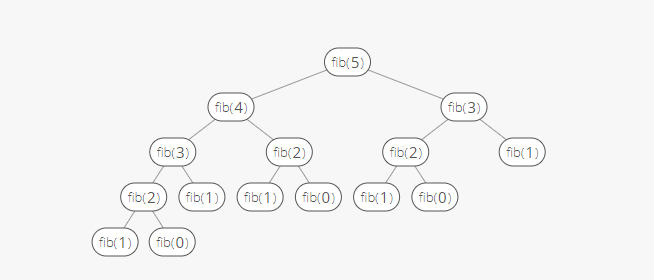
\includegraphics[height=5cm]{fib.png}
        \caption{Overlapping Sub-problems in determination of Fibonacci series}
        \label{fig:my_label}
    \end{figure}
\end{frame}

\section{A problem solved by dp}
\begin{frame}{We are going to see}
    \begin{itemize}
    \item A problem solved by dp 
    \end{itemize}
\end{frame}
\begin{frame}{Binomial Coefficient a.k.a C(n,r)}
    problem statement:{\color{red}ways to select}  r objects from n objects
regardless of the ordering
\end{frame}

\begin{frame}{Binomial Coefficient a.k.a C(n,r)}
    \begin{columns}
    \column{.5\textwidth}
    Naive approach : calculating $\frac{n!}{r!(n−r)!}$
    \column{0.5\textwidth}
    \begin{itemize}
        \item Problem : overflow will be caused calculating factorials, unsigned long long wouldn’t be enough. May be BigInteger would do but not efficient.
\item Solution : using dynamic programming.
    \end{itemize}
    \end{columns}
\end{frame}
\begin{frame}{C(n,r) having dynamic programming properties}
\textbf{Optimal Substructure:} C(n,r) can be recursively calculated using the formula,\\
$C (n,r ) = C (n −1,r −1) + C (n −1,r )$\\
with base cases, $C (n,0) = C (n,n) = 1$ and $C (n,1) = n$
\end{frame}
\begin{frame}{C(n,r) having dynamic programming properties}
\begin{center}
    \textbf{Overlapping Sub-problems: let n=5, r=2}
    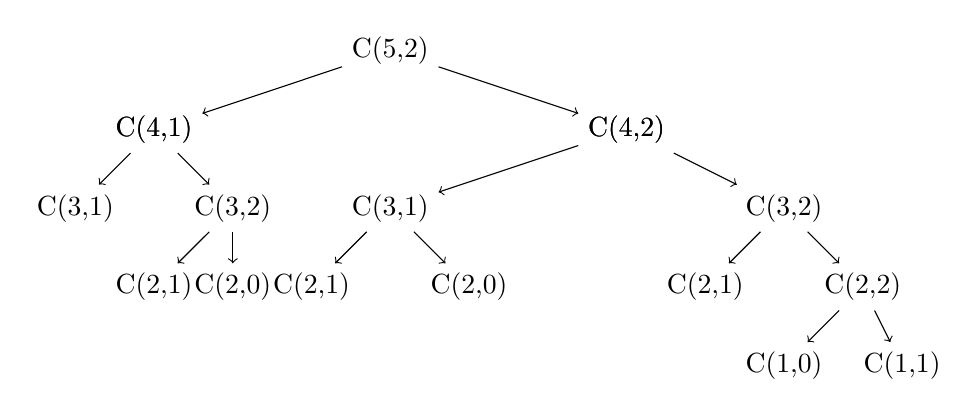
\begin{tikzpicture}
    \node(a) at (5,2)  {C(5,2)};
    \node(b) at (2,1)  {C(4,1)};
    \node(c) at (8,1)  {C(4,2)};
    \node(d) at (5,0)  {C(3,1)};
    \node(e) at (10,0)  {C(3,2)};
    \node(t) at (1,0)  {C(3,1)};
    \node(s) at (3,0)  {C(3,2)};
    \node(g) at (4,-1)  {C(2,1)};
    \node(h) at (6,-1)  {C(2,0)};
    \node(r) at (2,-1)  {C(2,1)};
    \node(m) at (3,-1)  {C(2,0)};
    \node(l) at (9,-1)  {C(2,1)};
    \node(k) at (11,-1)  {C(2,2)};
    \node(y) at (10,-2)  {C(1,0)};
    \node(w) at (11.5,-2)  {C(1,1)};
    \node(i) at (2,1)  {C(4,1)};
    \node(j) at (8,1)  {C(4,2)};
    \draw[->] (a) to (b);
    \draw[->] (a) to (c);
    \draw[->] (c) to (d);
    \draw[->] (c) to (e);
    \draw[->] (d) to (g);
    \draw[->] (d) to (h);
    \draw[->] (e) to (l);
    \draw[->] (e) to (k);
    \draw[->] (b) to (t);
    \draw[->] (b) to (s);
    \draw[->] (s) to (m);
    \draw[->] (s) to (r);
    \draw[->] (k) to (w);
    \draw[->] (k) to (y);
    \end{tikzpicture}
\end{center}
\end{frame}

\begin{frame}
    \begin{center}
    \begin{tabular}{|c||c|c|}
    \hline
    \multicolumn{3}{|c|}{Algorithm List}\\
    \hline
    Algorithm name & Time Complexity & Space Complexity\\
    \hline
    BFS & O ($|V |+ |E |$) & O ($|V |$)\\
DFS &  O ($|V |+ |E |$) & O ($|V |$)\\ \hline
Dijkstra & O ($|V |+|E |log |V |$) & O ($|V |+ |E |$)\\ \hline
Bellman Ford & O ($|V |∗|E |$) &  O ($|V |$)\\ \hline
Floyd–Warshall & O ($|V |^3$)  & O ($|V |^2$)\\ \hline
Edmonds–Karp & O ($|V |∗|E |^2$) & O ($|V |+ |E |$)\\\hline 
         \end{tabular}
\end{center}
\end{frame}





\end{document}
